\documentclass[a4paper,10pt]{article}

% Hier die Nummer des Blatts und Autoren angeben.
\newcommand{\blatt}{8}
\newcommand{\autor}{Merlin Steuer, Till Schander, Lennart Bergmann}

\usepackage{hci}

\begin{document}
% Seitenkopf mit Informationen
\kopf
\renewcommand{\figurename}{Figure}

\aufgabe{12}

\subsection{eCommerce-System: Amazon}
Amazon ist der wohl weltgröte Online-Handel. Es gibt kaum etwas, was man dort nicht kaufen kann, von Lebensmitteln über Alltagsgegenstände, Geschenke, Elektronik usw. Der Webshop von Amazon ist so aufgebaut, dass man sich wohl fühlt, wenn man einen größeren Supermarkt kennt. Die Artikel sind in Kategorien geordnet, welche man durchsuchen kann. Man kann auch einfach stöbern und sich von Amazon Produkte vorschlagen lassen, welche man interessant finden könnte. 
Öffnet man eine Kategorie, so wird eine Liste der beliebtesten Produkte dieser Kategorie angezeigt - ebenso, wie beliebte Produkte in Supermärkten i.d.R. vorn am Regal stehen, gut Sichtbar für den Kunden.

Das Konzept des Supermarktes wird natürlich bei Amazon erweitert durch verschiedenste Algorithmen zum Analysieren von Kaufverhalten und Vorschlagen von Produkten auf dieser Datenbasis.

\begin{itemize}
\item Die Supermarktregale: Produktkategorien

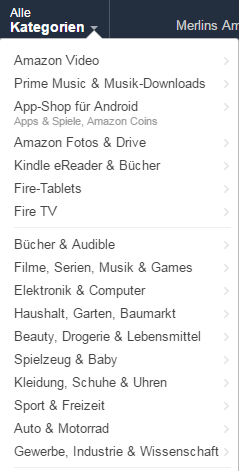
\includegraphics[scale=1]{images/kategorien.png}

Alle zusammenhängenden Produkte sind in so genannten Kategorien geordnet. Weiß man nur eine grobe Richtung dessen, was man kaufen möchte, so geht man zu diesem Regal bzw. betrachtet die Kategorie und durchstöbert sie. Möchte man ein genaues Produkt finden kann man auch innerhalb einer Kategorie suchen, um den Suchbereich einzugrenzen, ebenso wie man im Supermarkt zum Backwarenregal geht, wenn man Mehl sucht.

\item Der Einkaufswagen


\includegraphics[scale=1]{images/wagen.png}

Ähnlich wie man im Supermarkt während eines Einkaufs viele Artikel aussucht und in einen Einkaufswagen legt, lässt sich auch bei Amazon eine Menge von Artikeln für den späteren Kauf merken. Hier wurde die Einkaufswagenmetapher gewählt - man legt also Produkte virtuell hinein, welche man später dann bezahlen möchte.

\item Nämlich an der Kasse


\includegraphics[scale=1]{images/kasse.png}

In der Einkaufswagenansicht kann man \textit{zur Kasse gehen.} Man schiebt also seinen virtuellen Einkaufswagen zu einer Kasse, an der man seine Kreditkartendaten angibt, ähnlich als würde man im Supermarkt mit einer EC-KArte zahlen. Die Produkte werden dann zeitnah geliefert.
\end{itemize}

\subsection{Media-Player: VLC Media Player}
Der VLC Media Player ist einer der bekanntesten Open-Source Media Player. Er erlaubt es, Musikdateien vieler Formate, Videos, CDs und DVDs u.v.m. abzuspielen. Wir betrachten hier zunächst nur die Funktion des Musik Abspielens.

Der Media-Player möchte sich so bedienen lassen, wie das gute alte Stereo-Rack im Wohnzimmer. Ist eine Datei geöffnet, so möchte man, dass sich der Audiophile Stereoanlagenbesitzer möglichst zu Hause fühlt.

\begin{itemize}
\item Die Bedienelemente


\includegraphics[scale=1]{images/knoepfe.png}

Die Bedienelemente für Play, Pause, Stop, Forward/Rewind, Shuffle usw. sind alle mit Ikonen versehen, welche denen entsprechen, die man auf nahezug jeder Stereoanlage findet. Auch die Anordnung ist sehr ähnlich. Dadurch ist die Benutzung schnell und leicht erklärend. Sogar das lange Drücken der Vor- und Zurückspultasten funktioniert wie man es kennt. Drückt man ein mal kurz, springt der Titel einen weiter, hält man sie gedrückt, so spult man im aktuellen Titel vor und zurück.

\item Die Wiedergabeliste

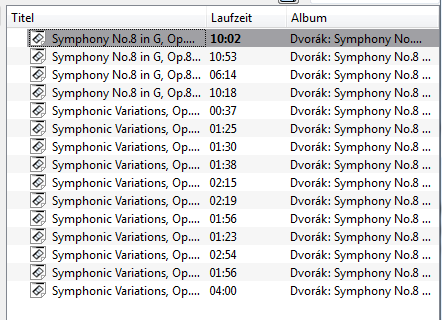
\includegraphics[scale=1]{images/liste.png}

Die Wiedergabeliste stellt das CD-Cover bzw. dessen Rückseite dar, auf welcher alle Titel einer Platte mit Namen, Reihenfolge und Spieldauer vermerkt sind. Oft sogar in einem Separaten Fenster (schließlich hält man die CD-Hülle ja auch neben der Anlage in der Hand) bekommt man so einen schnellen Überblick darüber, welche Titel die aktuelle CD noch zu bieten hat.

\item Der Equalizer

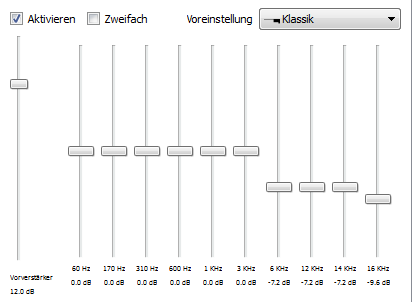
\includegraphics[scale=1]{images/eq.png}

Wer ein Audiophiler ist, der etwas auf sich hält, hat für jedes Genre und jeders Lautsprecher-Arrangement eine eigene Equalizer-Einstellung, welche auf seiner Anlage den besten Klang heraus kitzelt. Die typischen Schieberegler findet man noch heute in vielen Stereoanlagen-Racks. Der VLC-Mediaplayer bietet natürlich auch diese Funktionalität und bildet die Equalizer-Regler in einem Fenster so ab, wie man es aus der analogen Welt gewohnt ist.
\end{itemize}

\subsection{Soziales Netzwerk: Twitter}
Twitter ist ein Onlinedienst bei dem jeder der es möchte, alles was er tut, denkt oder mitbekommt in auf 140 Zeichen begrenzten Nachrichten der Welt mitteilen kann. Um alles mitzubekommen was ein bestimmter Nutzer mitteilt, kann man diesem folgen. Sollte einem eine Nachricht besonders gefallen, kann man diese mit einem Herzen versehen oder „re-tweeten“ um sie den eigenen „followern“ zu zeigen.

\begin{itemize}
\item

\includegraphics[scale=1]{images/twitter_startseite.png}

Als Symbol für die Startseite benutzt Twitter ein Haus, denn hier ist man „zuhause“. Die Startseite ist die erste Seite die man erreicht und von hier aus kann man alle anderen Funktionen und Bereiche nutzen.

\item

\includegraphics[scale=1]{images/twitter_nachrichten.png}

Für den Nachrichtendienst, bei dem man sich privat mit anderen Nutzern austauschen kann, benutzt Twitter ein Brief Symbol. Tatsächliche Briefe kann man dort nicht verschicken, trotzdem wird sofort klar, was sich hinter dem Symbol versteckt, auch wenn man Twitter in einer fremden Sprache verwendet.

\item 

\includegraphics[scale=1]{images/twitter_herz.png}

Um zu signalisieren, dass einem ein „Tweet“ gefällt, kann man es mit einem Herzen versehen. Herzen stehen für Liebe und gefallen, und wenn man etwas mit einem Herzen versieht so bedeutet das auch in der echten Welt, dass man dieses etwas mag. Auch hier wird jedem Nutzer ohne den Gebrauch von Sprache klar, was hinter der Funktion steckt.
\end{itemize}


\subsection{Dateimanager: Nautilus}
Der Dateimanager Nautilus ist für alle gängigen Linux-Distributionen verfügbar. Er erlaubt es mittels grafischer Oberfläche die Ordner- und Dateistruktur auf Festplatten anzuzeigen und zu verändern. Der Dateimanager wirkt durch die Wahl mehrerer Metaphern wie eine Digitale Version eines Aktenschranks.

\begin{itemize}
\item Datei- und Ordnericons

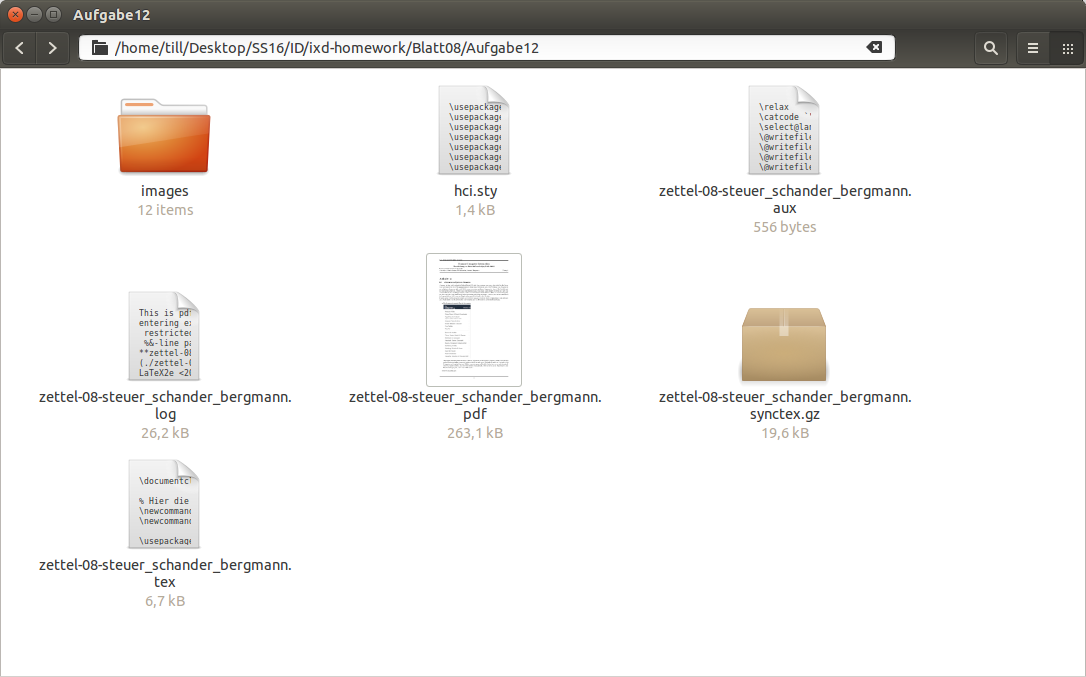
\includegraphics[scale=0.395]{images/icons1.png}

Am prominentesten sichtbar wird die Aktenschrank-Metapher anhand der Datei- und Ordnericons sichtbar. Ordner werden hier durch das Abbild eines Hängehefters repräsentiert. Die Dateien in einem solchen Ordner sehen aus wie einzelne Blätter. Dies ist sinnvoll, da Hängehefter genutzt werden um einzelne Blätter zu lagern. Die „Blätter“ sind nicht einfach leer, sondern zeigen, wie in echt, ihren Inhalt. Manche Dateien bekommen eigene Icons. So sehen zum Beispiel komprimierte Dateien wie gepackte Umzugskartons aus.


\item Lesezeichen

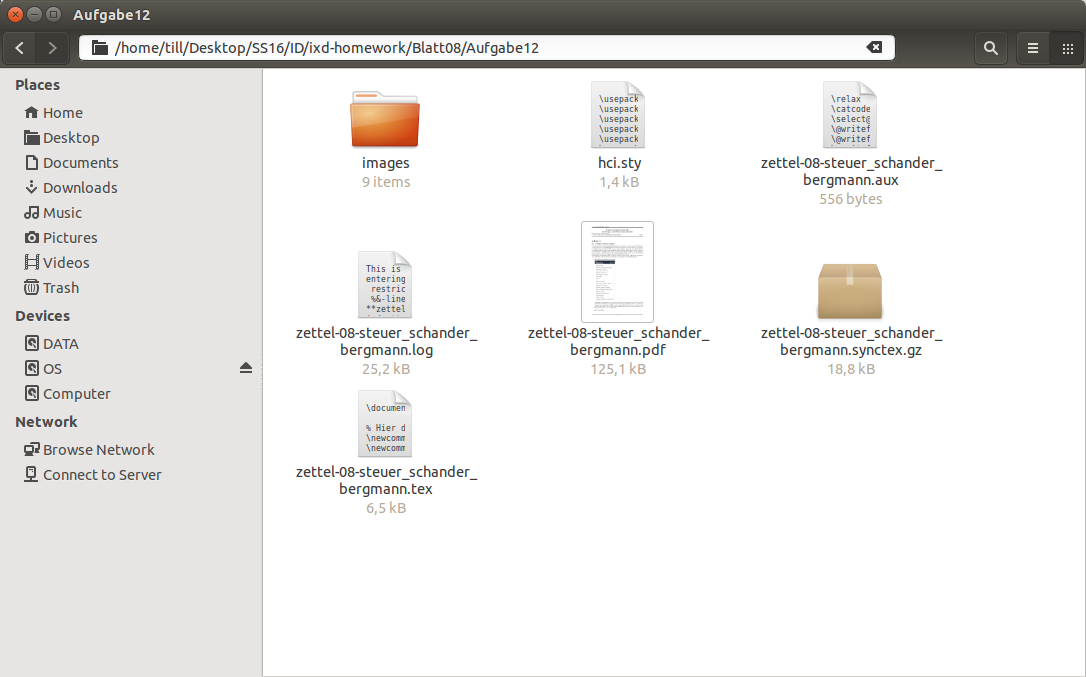
\includegraphics[scale=0.395]{images/icons2.png}

In Nautilus können verschiedene Lesezeichen eingeblendet und verwaltet werden. Diese ermöglichen ein schnelleres Navigieren durch das Dateisystem. Die Lesezeichen werden in der Seitenleiste von Nautilus „Orte“ genannt, als ob sie echte Orte in einem Büro/Schrank wären. Standard-Orte bekommen zudem eigene Icons, welche zumeist das Abbild eines physischen Objekts sind.


\item Suche

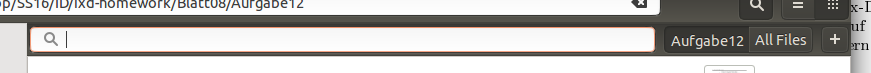
\includegraphics[scale=0.49]{images/icons3.png}

Nautilus kommt mit einer integrierten Suche. Diese ermöglicht es schnell Ordner und Dateien anhand ihres Namens zu finden. Das Icon für die Suche ist eine Lupe, da Lupen verwendet werden, um nur schwer sichtbare Dinge besser sichtbar zu machen. Außerdem erlaubt die Suchfunktion das Suchen ab einem bestimmten Ordner tiefer gehend. Bezogen auf die Aktenschrank-Metapher ist dies, als würde der Nutzer nur in einem bestimmten Abschnitt des Schranks suchen.

\end{itemize}

\end{document}
